%%%%%

\documentclass[letterpaper, 10 pt, conference]{ieeeconf}  % Comment this line out if you need a4paper
\usepackage{graphicx}

\usepackage{color}
\definecolor{orange}{rgb}{1,0.5,0}
\definecolor{mygreen}{RGB}{55,230,55}
\newcommand{\bobby}[1]{\textcolor{blue}{(Bobby: #1)}}
\newcommand{\bbc}[1]{\textcolor{blue}{(Bobby: #1)}}
\newcommand{\lingfeng}[1]{\textcolor{orange}{(Lingfeng: #1)}}
\newcommand{\richard}[1]{\textcolor{red}{(Richard: #1)}}
\newcommand{\rap}[1]{\textcolor{red}{(Richard: #1)}}
\newcommand{\daniel}[1]{\textcolor{teal}{(Daniel: #1)}}


\IEEEoverridecommandlockouts                              % This command is only needed if 
                                                          % you want to use the \thanks command
\overrideIEEEmargins                                      % Needed to meet printer requirements.

%In case you encounter the following error:
%Error 1010 The PDF file may be corrupt (unable to open PDF file) OR
%Error 1000 An error occurred while parsing a contents stream. Unable to analyze the PDF file.
%This is a known problem with pdfLaTeX conversion filter. The file cannot be opened with acrobat reader
%Please use one of the alternatives below to circumvent this error by uncommenting one or the other
%\pdfobjcompresslevel=0
%\pdfminorversion=4

% See the \addtolength command later in the file to balance the column lengths
% on the last page of the document

% The following packages can be found on http:\\www.ctan.org
%\usepackage{graphics} % for pdf, bitmapped graphics files
%\usepackage{epsfig} % for postscript graphics files
%\usepackage{mathptmx} % assumes new font selection scheme installed
%\usepackage{times} % assumes new font selection scheme installed
%\usepackage{amsmath} % assumes amsmath package installed
%\usepackage{amssymb}  % assumes amsmath package installed

\title{\LARGE \bf
Emergency Clinical Procedure Detection With Deep Learning
}


\author{Lingfeng Li$^{1}$, Richard A. Paris$^{1}$, Conner Pinson$^1$, Yan Wang$^1$, Joseph Coco$^2$, Jamison Heard$^3$,\\
Julie A. Adams$^4$, \textit{Senior Member, IEEE}, Daniel V. Fabbri$^{2}$, and Bobby Bodenheimer$^{1}$, \textit{Senior Member, IEEE}
\thanks{This work was supported by the Department of Defense Contract Number W81XWH-17-C-0252 from the CDMRP Defense Medical Research and Development Program.}% <-this % stops a space
\thanks{$^{1}$Department of Electrical Engineering and Computer Science,
        Vanderbilt University, Nashville, Tennessee
        }%
\thanks{$^{2}$Vanderbilt University Medical Center, Nashville, Tennessee
        }%
\thanks{$^{3}$Department of Electrical and Microelectronic Engineering, Rochester Institute of Technology, Rochester, NY
        }%
\thanks{$^{4}$Collaborative Robotics and Intelligent Systems Institute, Oregon State University, Corvallis, Oregon
        }%
\thanks{Corresponding author email: bobby.bodenheimer@vanderbilt.edu}
}


\begin{document}



\maketitle
\thispagestyle{empty}
\pagestyle{empty}


%%%%%
\begin{abstract}

Information about a patient’s state is critical for hospitals to provide timely care and treatment. Prior work on improving the information flow from emergency medical services (EMS) to hospitals demonstrated the potential of using automated algorithms to detect clinical procedures. However, prior work has not made effective use of video sources that might be available during patient care. In this paper we explore the use convolutional neural networks (CNNs) on raw video data to determine how well video data alone can automatically identify clinical procedures. We apply multiple deep learning models to this problem, with significant variation in results. Our findings indicate performance improvements compared to prior work, but also indicate a need for more training data to reach clinically deployable levels of success. 

\end{abstract}

%%%%%%
\section{INTRODUCTION}

Possessing and communicating accurate patient information is critical to achieving optimal medical outcomes. Unfortunately, too often emergency medical services (EMS) does not communicate complete information to a treating hospital [1]. This lack of communication can lead to inferior patient outcomes as the initial triage of a patient's condition can be done incorrectly at the receiving hospital [2]. This paper discusses a component of a noninvasive system that could potentially detect automatically what clinical procedures have been performed on a patient. Ideally, this system would supplement current care procedures by providing improved information on patient care to receiving hospitals, with the goal of improving a patient's initial triage level.

Heard et al.~[2] made initial forays into this area by presenting a system that employed information from multiple types of sensors, including video, to categorize clinical procedures. Building on work in human activity recognition from multiple sensors [3], this work used contextual information provided by video sources to locate a medic's hands.  Based on this location and other sensor information, this work represented a first step at clinical procedure identification. Its highest accuracy was achieved when the algorithm algorithm knew the active body region to which the procedure was applied (18\% accuracy without body region knowledge and 40\% accuracy with perfect body region knowledge).

This paper represents a new effort into this problem and only uses video data. It is motivated by recent developments in video classification and recognition in deep learning [4-6]. We use convolutional neural networks (CNNs) on raw video data to detect different clinical procedures performed during EMS transport. We attempted this because we want to see how far video data alone can take us, and to assess how much video data is necessary to achieve adequate performance from these data sets alone. There is an operational advantage from video data in that would not require paramedics to wear sensors. On the other hand, video data suffers from occlusion problems and noise due to lighting changes, and thus may have other difficulties for learning algorithms. Nonetheless, understanding how well video data by itself can work for classification is an important step in the development of an automatic clinical procedure system.

\section{Related Work}

Karpathy et al. [8] demonstrated the effectiveness of convolutional neural networks (CNN) on video classification tasks. They explored four different models for fusing information over temporal dimension through networks. All models exhibited strong capabilities for classifying video clips. Of their approaches, we primarily explored the single frame approach and the late fusion approach, as illustrated in Figure~1. 
\begin{figure}[!htb]
        \center{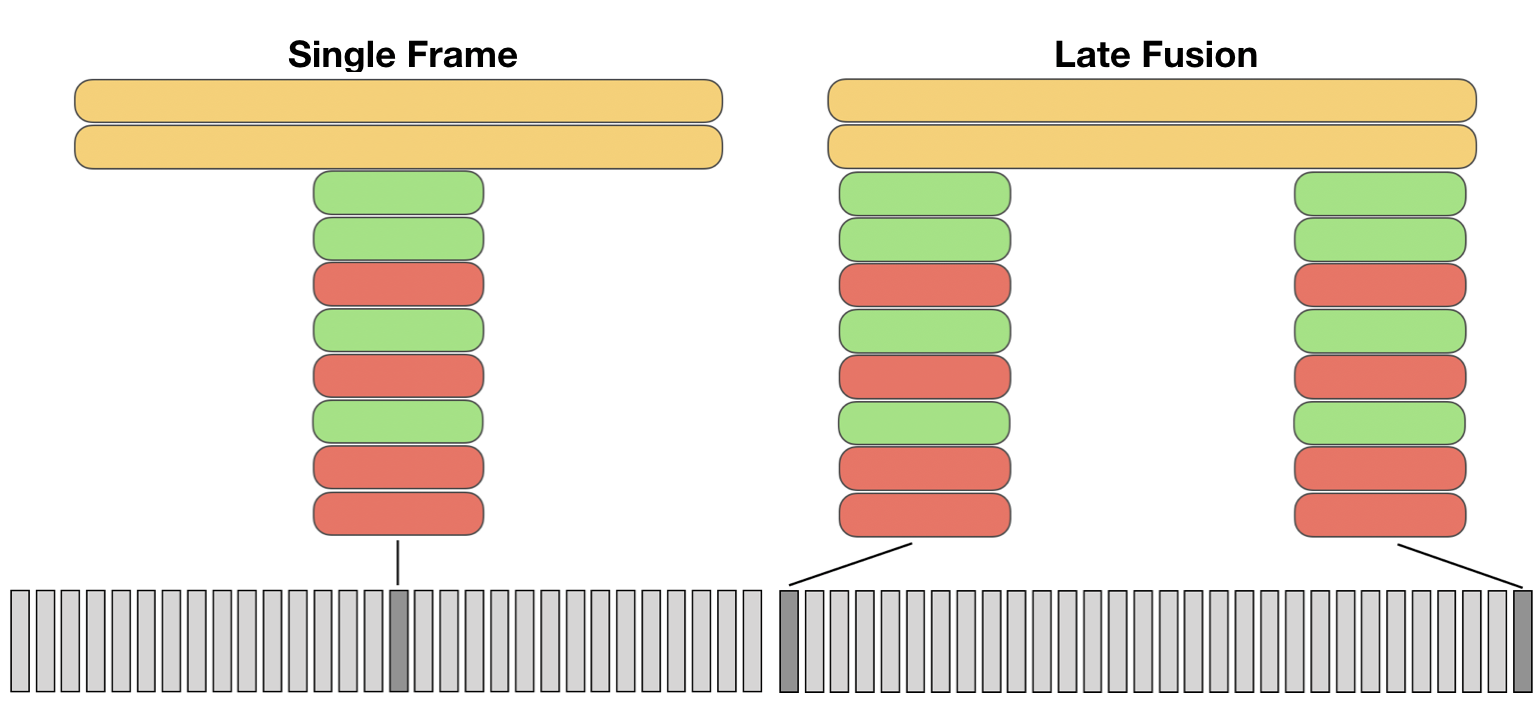
\includegraphics[width=25em]
        {./Fg1.png}}
        \caption{\label{fig: sampling} Illustration of the Single Frame and Late Fusion Structures. The single frame model classifies based on one frame of the video stream (depicted at the bottom), whereas the late fusion model uses multiple temporally close frames. Red and green boxes together represent a mixture of convolutional layers and utility layers; yellow boxes represent fully connected layers. }
      \end{figure}
      
Ng et al.~[6] and Donahue et al.~[5] demonstrated the use of Long Short Term Memory (LSTM) for video classification tasks. These two groups of researchers processed individual frames with CNNs to aggregate information from frame data, and then the aggregated data is passed to the LSTM network for information summation. Results shown by Ng et al. and Donahue et al. suggest that LSTMs can achieve better video classification results than CNN methods if tuned well.


\section{Data Collection and Dataset Creation}

All experimental data were collected in the Center for Experiential Learning and Assessment (CELA) at the Vanderbilt University Medical Center [7]. Seven subjects with medical training performed 24 different procedures (Table 1) with varying amounts of repetition. Subjects performed the procedures on realistic medical mannequins that are commonly used for medical training. To collect video data four cameras were placed at different locations (Figure~2). They were positioned to capture as much of the procedure as possible and to ensure that the important parts of the procedure were always captured. Camera 2 (C2) was placed to emulate a ceiling mounted camera in an ambulance. Each camera collected video with a resolution of 3840 $\times$ 2160. This paper analyzed only C2 data as it was sufficient to ensure the mannequin, subject, and action were always visible.

%Paris \textit{et al}. [7] in collaboration with Vanderbilt University Medical Center collected clinical procedures applied to emergency care mannequins. 24 categories of procedures were performed by seven paramedics (subjects) to medical mannequins and collected by four cameras placed at different locations. All category labels can be found at Table 1. The positioning of the cameras [7] relative to the patient is shown in Figure 2, and each camera shot 4K video at 24 fps. This research will make use of all video footage collected at position C2. 

\begin{figure}[!htb]
        \center{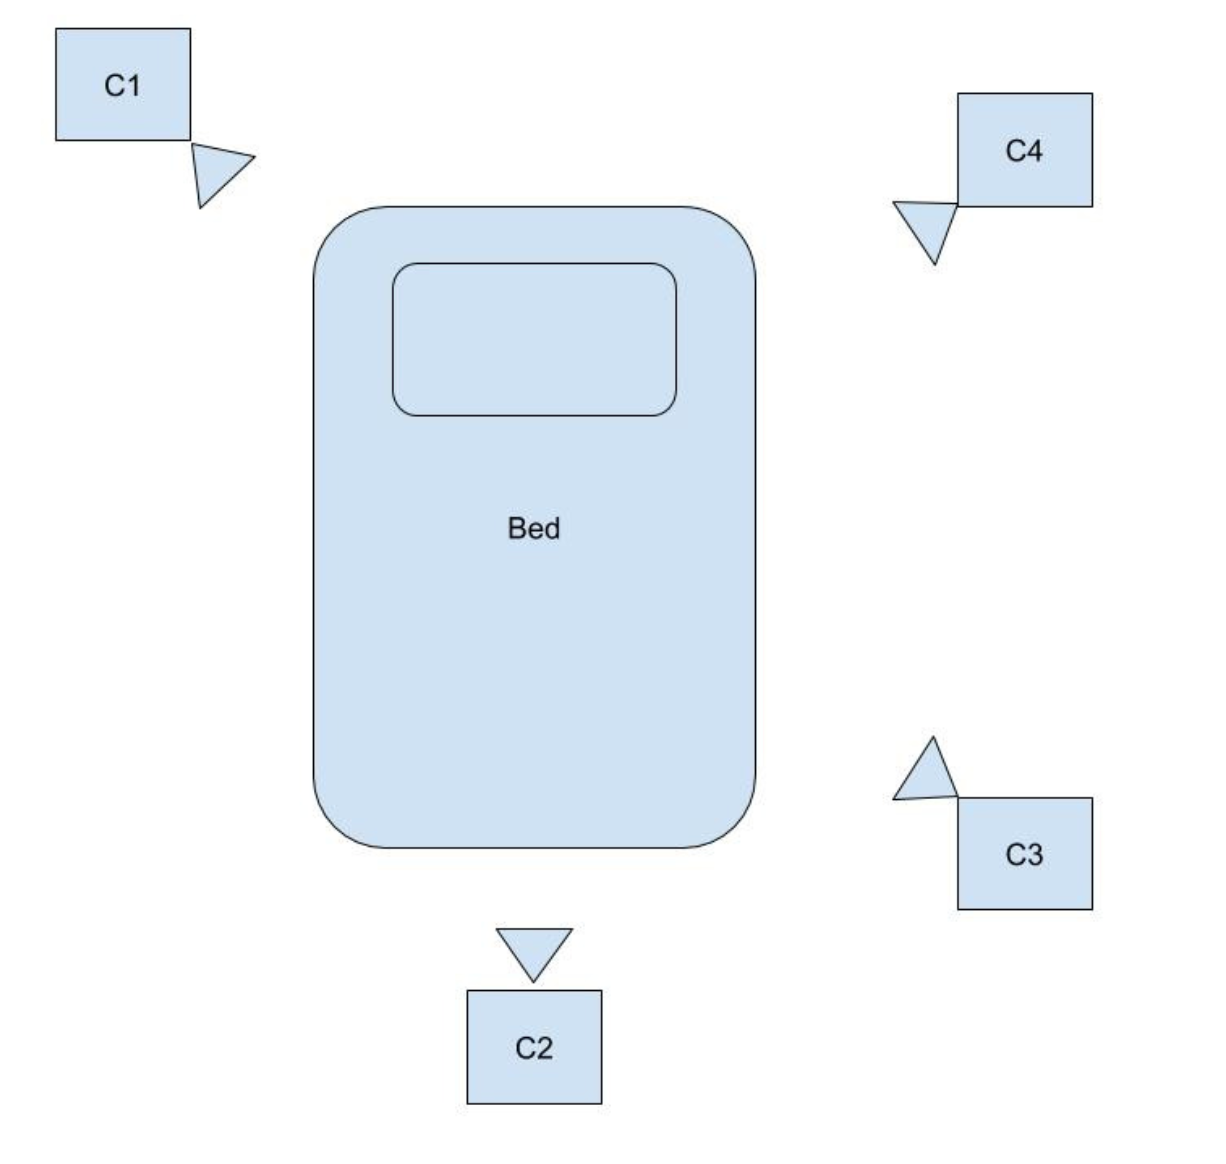
\includegraphics[width=25em]
        {./Fg2a.png}}
        \caption{\label{fig: camera positions} Positioning of the four cameras used during data collection, as described in Paris et al.~[7]. }
      \end{figure}
      
\begin{table}[!htb]
\begin{center}
 \begin{tabular}{||l l l||} 
 \hline
Administer Medication & Bagging & Blood-Pressure Cuff  \\ [0.5ex] 
 \hline
Chest-tube Prep & Chest-tube & Combat Tourniquet  \\ 
 \hline
CPR (Compression) & CPR (Breath) & Swab Area with Alcohol  \\ 
 \hline
Intubation & IO Line & IV Line  \\ 
 \hline
King Airway & Oral Airway & Pulse-OX  \\
\hline
Draw Medication & ECG Leads & Vital Checking  \\
\hline
Combat Gauze& Suturing& IM Administration \\
\hline
 IV Tourniquet & Splinting & Wrap Head Wounds \\
\hline

\end{tabular}
\caption{Table 1: Categories of clinical procedures. Abbreviations: IM -- intramuscular; ECG -- electrocardiogram; IV -- intravenous therapy; IO -- intraosseous; OX -- oxygen.}
\end{center}
\end{table}

The collected video data were split into individual frames and each frame was assigned a category. Frames during which no procedure occurred were discarded. Each frame was cropped to reduce data size and eliminate extraneous information. Figure~3 shows the lines along which cropping occurred. The resulting frames were then resized to $256 \times 256$ pixels. In addition to the procedure name, each frame was labeled with the subject number and procedure occurrence as each procedure occurred multiple times. 

%Video data were presented as 8 minutes 53 seconds clips. Video clips were concatenated into single video roll and exported as frame data at 30 frames per second. In order to center the subject and fit in memory, each frame is cropped according to the plan shown in figure 3, and then resized to 256*256. For videos and frame data that are vertically flipped, the resizing plan is accordingly mirrored and applied. 



%Frame data are then sorted according to subject and procedure categories. For temporal relations, frame data are further sorted by the occurrence of each procedure, because each procedure may occur multiple times during a video. Table 2 is a sequence of medical procedures excerpt from subject 2, procedure \textit{Draw Medication}, \textit{IV Line}, and \textit{Swab Area with Alcohol} (labeled with *) appeared twice in the sample segment, and thus they are respectively counted as different samples within the subject dataset.

 \begin{figure}[!htb]
        \center{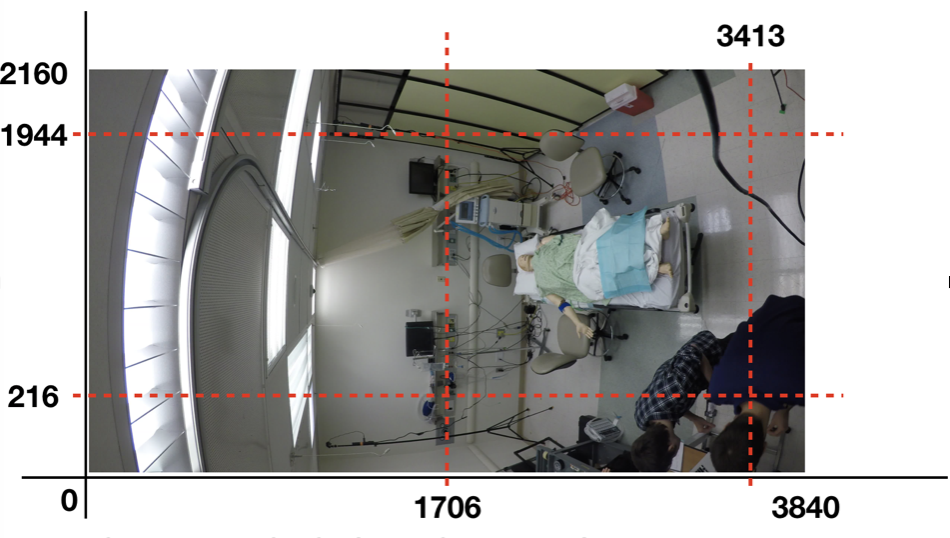
\includegraphics[width=25em]
        {./Fg3.png}}
        \caption{\label{fig: resizing plan} Image cropping plan for frame data --- only the central region is kept.}
      \end{figure}
      
% \begin{table}[!htb]      
% \begin{center}
%  \begin{tabular}{||l l l||} 
%  \hline
% Procedure & Start Time & Stop Time \\ [0.5ex] 
%  \hline\hline
% CPR (Compression) & 477.016 & 1087.163 \\ 
%  \hline
% CPR (Breath) & 1087.163 & 1191.598 \\ 
%  \hline
% CPR (Compression) & 1191.598 & 1777.622 \\ 
%  \hline
% CPR (Breath) & 1777.622 & 1918.596 \\
% \hline
% ... & ... & ...  \\
% \hline
% Chest-tube Prep & 128455.330 & 129217.812 \\
% \hline
% Chest-tube & 129217.812 & 130996.678 \\
% \hline
% ... & ... & ...\\
% \hline
% Chest-tube Prep & 205292.595 & 207387.941\\
% \hline
% Chest-tube & 207387.941 & 210059.237\\
% \hline

% \end{tabular}
% \caption{Table 2: An Exampring One Video. Remove table 2 from paper. It's not helpful}
% \end{center}
% \end{table}

Of the data set composed of seven subjects, data from 
five subjects were used for training, one for validation, and one for training. We performed 5-fold cross validation by rotating the subject used for validation and for testing. We chose to fold on subjects as we want to ensure the model generalizes to new and different medics performing the procedures.

%Datasets are created according to subjects. Training dataset consists of data from five subjects, while validation and testing datasets each contains data from one of the remaining two subjects. 5-fold cross validation datasets are created by rotating subjects used for validation and testing.

Subjects in this experiment completed each procedure a randomized number of times and the time to complete each procedure varied leading to imbalanced classes. Class sizes ranged from 3,000 frames to 60,000 frames. To ensure the model does not overfit to one category and every class is equally represented the data was either downsampled or upsampled to approximately 8,000 frames. To downsample, approximately 8,000 random frames were selected and others discarded. To upsample, we duplicated each frame; then, if the upsampled category contained more than 8,000, it was downsampled as in the other categories. For example, in the fold 2 training set, the category \textit{Pulse-OX} contained 3544 frames, and all frames were duplicated to reach 7088 frames (approximately 8000). Category \textit{Chest-tube Prep} contained 6480 frames. We duplicated these frames and selected 8000 random frames, discarding the rest. 

Validation and testing sets were balanced similarly with only the target number of frames changing. Our target was chosen so that only 15\% of the classes would require duplication. The other 85\% would then require downsampling. For each fold a different value was chosen based on the size of the categories in that validation or testing fold.

%CNN models use frame data for training. However, frame data available for each category is different, ranging from as few as 3,000 frames to as abundant as 60,000 frames for training dataset. To ensure the model does not heavily favor one category over another, each category randomly select 8,000 frames from available data. For categories with frame data less than the 10,000 threshold, frame data are duplicated twice. For example, one category with 3,000 frames will be duplicated to 6,000 frames, and all 6,000 frames will be used; another category with 6,000 frames will be duplicated to 12,000 frames, and then 8,000 of the frames will be randomly selected from the pool. 

%The same disproportion of size between categories also happens to validation dataset and testing dataset. In order to present a more representative capability of models at accurately classifying categories, validation datasets and testing datasets are balanced as well. Threshold of maximum sample count for all categories is selected so that at least 85\% of the categories have data more than the threshold. For example, for Fold 3, we select 2,000 as the standard size of all testing and validation categories, because 20 categories (85\% of total categories) have size larger than 2,000.

%You need to explain the paragraph above and below in more detail I don't understand either

The previous balancing plan applies to two of the CNN models we test in this paper, the so-called ``main model'' (Section~\ref{sec:mainmodel}) and ``variant 1''  (Section~\ref{sec:variant1}). A third model, ``variant 2'' (Section~\ref{sec:variant2}), makes use of temporal relationships and has additional data inputs. For this model,  we reduce our data size by resampling each session at 6 fps. In other words we choose frames 0, 5, 10, etc. To combat class balance issues we need to include more incidences of categories with lower representation. To do this we divide our categories into large, medium, and small. Large categories only resample once, medium categories resample an additional two times, and small categories an additional four times. These additional resamplings are offset from 1 to 4 frames from the first frame which gives us slight differences in our samples.

%For models making use of temporal relationships between frame data, data samples are counted by sessions, and all sessions will be sampled at 6 frames per second (FPS), so session count can be augmented by 2 to 3 times, and similar threshold for sample count is enforced so that at least 60\% of the categories have sample count more than the threshold.

Our analysis system is built on Keras, Python's deep learning library.\footnote{https://keras.io/} Keras' built-in image augmentation framework helped increase the variability in the data. The brightness, rotation, zoom were all randomly modified. Images were randomly shifted vertically or horizontally, and could randomly be flipped vertically or horizontally. For models using temporal relationships, the same augmentations were applied to each related frame. 

%As a measurement for data augmentation and also a method to address the similarity between cloned frame data and sessions, image data augmentation from Keras is used for all training data. Methods such as rotation, width shift, height shift, brightness, zoom, horizontal flip, and vertical flip are all randomly applied to frame data to create variations. For models that uses temporal relationships, methods and parameter applied to each session are the same but varies on a session to session basis.


\section{Methods}\label{sec:methods}
The models in this section are largely based on InceptionV3 due to its success in image recognition tasks [10]. All training is done starting with the pretrained imageNet weights for low-level feature detection. For each fold the model was trained until a baseline validation accuracy was reached and the testing accuracy measured. This occurred three times per fold with the highest testing accuracy being recorded.

%We develop and tweak our models first on one fold dataset and try to prove the generalizability of model through 5-fold cross validation. We create our models mainly based on InceptionV3 due to its high performance and popularity in image recognition tasks. We train our models with imageNet weight-initialization, because imageNet weights generalized low-level details well.

%All models are trained with mini batch of size 64 and early stopping point is picked based on validation accuracies. With in each fold, the models are trained with weight initialization three times, and highest achieving accuracy is recorded.
\begin{figure}[!htb]
        \center{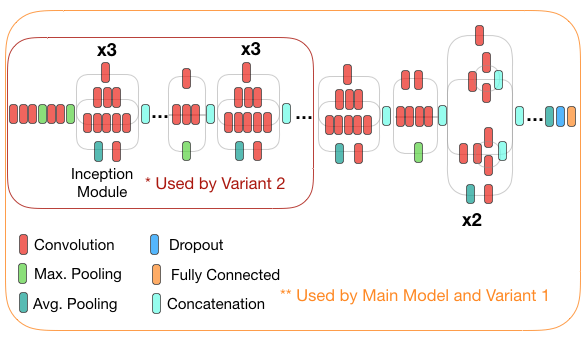
\includegraphics[width=25em]
        {./Fg3xc.png}}
        \caption{\label{fig: InceptionV3} A Compressed View of InceptionV3 [10]. The portion used by the main model and variant 2 are depicted with the orange and red lines, respectively.}
     \end{figure}
 \begin{figure}[!htb]
        \center{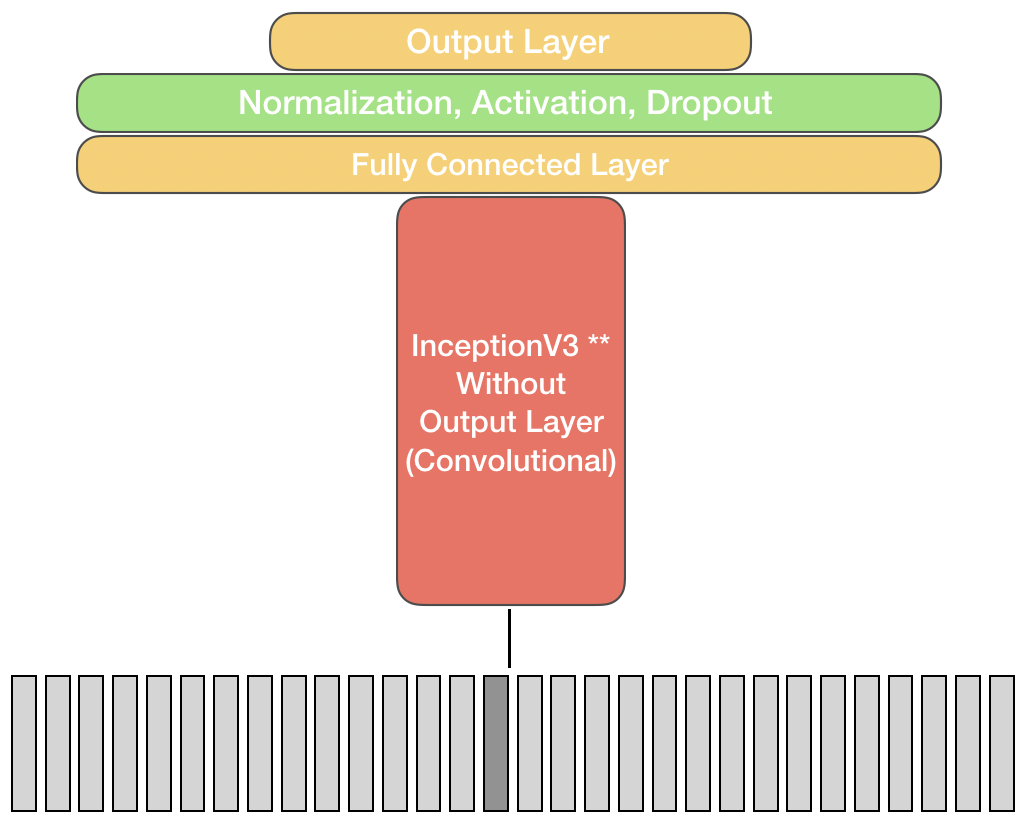
\includegraphics[width=25em]
        {./Fg3x.png}}
        \caption{\label{fig: Main Model} An Illustration of main model, a direct adaptation of InceptionV3. A red box represents the part of model taken from InceptionV3 (portion of the model marked with ** in Figure~4); a yellow box represents dense layers; a green box represents utility layers.}
      \end{figure}
      
\subsection{Main Model: Full Inception Model with Single Frame}\label{sec:mainmodel}

Karpathy et al. [8] demonstrated that a single frame was sufficient to achieve a high accuracy (40\%) in large datasets such as the UCF-101 and the Sport1M datasets. Those datasets are more complex than the clinical procedure dataset. The InveptionV3 architecture is a popular choice for deep learning image recognition tasks and we choose to use it as the basis of our network. Given the similarity of domains (action recognition), we expect similarly strong results. The clinical procedure dataset is smaller than similar datasets so the pretrained ImageNet weights were used to reduce training time and increase performance. Figure~5 is an illustration of this architecture, which we call our main model. Our model is made of the InveptionV3 architecture without the final output layer. Instead we place a fully connected layer, normalization, activation, dropout, and a second fully connected layer to adapt the model to our problem.

%Karpathy et al. [8] demonstrated that by simply analyzing data from one frame, their single frame model can achieve 40\% accuracy or higher in large scale datasets such as UCF-101 and Sport1M. The clinical procedure dataset is a much simpler dataset than either of UCT-101 or Sport1M dataset, and InceptionV3 has much higher model capacity than the single-frame model used by Karpathy et al. Thus we expect that by simply applying single-frame InceptionV3, we expected similar results given the similarity in domains. \rap{I don't think we should say we expect at least 40\% accuracy. Just because it got 40\% in one domain doesn't mean it will in ours. We should just say we expected similar results given the similarity in domains. (no numbers)}\bbc{I agree.}\lingfeng{Slightly modified, please review}

\subsection{Variant 1: Full Inception Model with Combined Categories}\label{sec:variant1}

In the application domain for which we are training our recognition models, many
 of the procedures, while different actions, have temporal or physical associations with each other. For example, \textit{Chest-tube Prep} must occur before \textit{Chest-tube} and \textit{CPR (Breath)} alternates with \textit{CPR (Compression)}. In this variant we explore combining the \textit{CPR (Breath)} and \textit{CPR (Compression)} categories, as it is possible that we might get improved performance by grouping these associations manually rather than letting the algorithm determine them automatically.  In particular, the main model commonly confused these two procedures and the goal is to remove that confusion and look for features common to both procedures.

%Some of the categories, such as \textit{CPR (Breath)} and \textit{CPR (Compression)}, \textit{Chest-tube Prep} and \textit{Chest-tube} have different actions. However, while their actions are different, it is not helpful to know in detail whether \textit{CPR (Breath)} or \textit{CPR (Compression)} is done, or whether \textit{Chest-tube Prep} or \textit{Chest-tube} is done. 

%We explore the effect of combining similar categories. While leave everything else to be the same, we only combine \textit{CPR (Breath)} and \textit{CPR (Compression)}, and we want to compare the result of one category combination with no combination.

\subsection{Variant 2: Partial Inception Model with Late Fusion}\label{sec:variant2}
Popular datasets,  such as UCF101, Sport1M, or Youtube8M, cover a wide variety of topics, fields, and activities. Most of classes can be distinguished with one single frame. One problem we face is that some of the categories in the clinical procedure dataset, due to the similarity in context and equipment, cannot be easily distinguished from each other with a still image. 

 \begin{figure}[!htb]
        \center{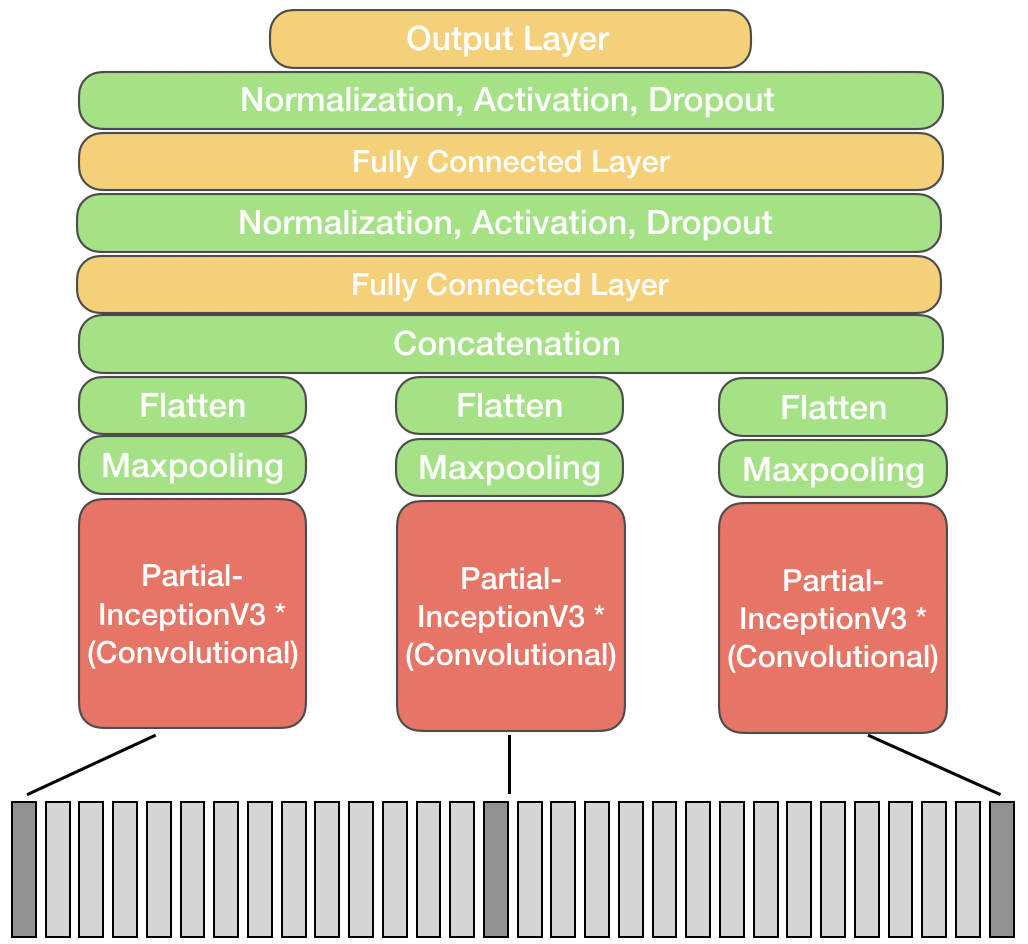
\includegraphics[width=25em]
        {./Fg4.png}}
        \caption{\label{fig: Illustration of Late Fusion} 
        The variant 2 model, a CNN model using the concept of Late Fusion.  Red boxes represent the part of model taken from InceptionV3 (portion marked with * in Figure~4); yellow boxes represent dense layers;  green boxes represent utility layers; light and dark grey boxes represent available and selected frame data.}
      \end{figure}

To overcome this difficulty, we took inspiration from Late Fusion, and sample the video three times across a one second span: each data sample consists of the first frame of the second, the middle frame of the second, and the last frame of the second (1st frame, 15th frame, and 30th frame). Figure~6 is an illustration of our variant 2 (late fusion) model that takes advantage of both frame information and temporal information between frames. We first use convolutional layers and Inception Modules [10], which concatenate the results of different sizes of convolutional filters, to summarize information from each frame sample. Frame information is then fused to temporal relations in the top fully connected layers. Lastly, the output layer classifies clinical procedure based on given frame information and temporal information. 
The standard InceptionV3 model is further pared down to use only six inception modules as a feature extractor. Three equivalent copies with shared weights of those six modules were created. These three were each fed into a separate maxpooling and flatten layer before being concatenated and fed through a series of layers as shown in Figure~6. 

%The three lower branches of variant 2 are essentially based on the first half of the InceptionV3 with weights initialized to pre-trained imageNet. The three branches are the exact same copy of each other, and they share the same weights with each other before and after training.  \bbc{What are we supposed to take away from Figure 4? You haven't explained to the reader what any of the blocks, e.g., flatten, fully connectd layer, mean. If you can't do that in a concise and easily understood way, then you need a different figure. As it stands this figure is confusing and really only informs people who already know what the late fusion model is as to what's going on.} \lingfeng{ I'm not sure if my explanation is better this time, I added more details in the graph, and a bit more explanation in the paper, but I don't know if I should talk about maxpooling, flatten, concatenate, etc.}

\section{Results}

\begin{table}[!htb]
\begin{center}
 \begin{tabular}{||l c c c ||} 
 \hline
Fold & Main Model & Variant 1 & Variant 2  \\ [0.5ex] 
 \hline\hline
Fold 1 & 53.593\% & 57.798\% & 47.402\%  \\ 
 \hline
Fold 2 & 42.398\% & 45.842\% & 50.506\% \\ 
 \hline
Fold 3 & 46.813\% & 44.975\% & 51.053\% \\ 
 \hline
Fold 4 & 44.525\% & 48.197\% & 61.770\% \\ 
 \hline
Fold 5 & 52.673\% & 53.504\% & 55.114\% \\ 
 \hline
Avg. Acc& 48.000\% & 50.063\% & 53.169\% \\ 
 \hline
\end{tabular}
\caption{Table 2: The  testing accuracy of the three models across various folds and the resulting accuracy over all folds.}
\end{center}
\end{table}

\begin{table}[!htb]
\begin{center}
 \begin{tabular}{||l c c c  ||} 
 \hline
 & Main Model & Variant 1 & Variant 2  \\ [0.5ex] 
 \hline\hline
Administer Medication & 36.743\% & 31.083\% & 12.222\%  \\ 
 \hline
Bagging & 66.476\% & 62.873\% & 90.371\% \\ 
 \hline
Blood-Pressure Cuff & 39.218\% & 44.975\% & 24.572\% \\ 
 \hline
Chest-Tube & 58.013\% & 59.649\% & 72.113\% \\ 
 \hline
Chest-Tube Prep & 0\% & 0.422\% & 0\% \\ 
 \hline
Combat Gauze & 45.668\% & 35.321\% & 35.576\% \\ 
 \hline
 Combat Tourniquet & 98.661\% & 94.474\% & 94.177\% \\ 
 \hline
CPR (Breath) & 55.593\% & 72.120\% & 31.827\% \\ 
 \hline
CPR (Compression) & 43.424\% & N/A & 32.649\% \\ 
 \hline
 Draw Medication & 7.099\% & 7.272\% & 4.382\% \\ 
 \hline
 ECG Leads & 56.050\% & 84.432\% & 69.910\% \\ 
 \hline
 IM Administration & 25.591\% & 18.931\% & 8.593\% \\ 
 \hline
 Intubation & 32.750\% & 51.789\% & 13.106\% \\ 
 \hline
 IO Line & 63.121\% & 67.852\% & 68.993\% \\ 
 \hline
 IV Line & 60.799\% & 58.810\% & 80.794\% \\ 
 \hline
 IV Tourniquet & 39.007\% & 35.527\% & 23.977\% \\ 
 \hline
 King Airway & 31.208\% & 47.505\% & 13.705\% \\ 
 \hline
 Oral Airway & 33.761\% & 41.290\% & 56.685\% \\ 
 \hline
 Pulse-OX & 35.269\% & 16.118\% & 10.000\%\\ 
 \hline
 Splinting & 79.053\% & 95.100\% & 61.038\% \\ 
 \hline
 Suturing & 54.862\% & 49.358\% & 40.258\% \\ 
 \hline
 Swab Area W/ Alcohol & 6.189\% & 19.863\% & 2.920\% \\ 
 \hline
 Vital Checking & 46.600\% & 24.816\% & 37.195\% \\ 
 \hline
 Wrap Head Wound & 92.089\% &93.817\% & 81.202\% \\ 
 \hline
 Total & 47.474\% & 49.113\% & 41.731\% \\ 
 \hline
\end{tabular}
\caption{Table 3: The  testing accuracy by category from the 5-fold cross validation. }
\end{center}
\end{table}


%Discuss the validity of testing results
The results of the 5-fold cross validation can be found in Table 2 and the  categorical accuracy of models across 5-fold cross validation can be found in Table 3. Table 3 is computed by calculating the accuracy for each category for each fold and then averaging the categorical data across 5 folds, so that each experiment is given same weight in the result. Entry \textit{CPR (Breath)} for variant 1 gives the accuracy for the combined CPR category.  Table~2 is the traditional way of calculating accuracy for a cross-validation; however, Table~3 gives a better idea of the performance of the classifiers across each category, and since it balances each category equally, it gives a better overall indicator of performance.

The main model and variant 1 use single frame data for classification, while variant 2 uses 3 frames evenly spaced from 1 second of data for procedure detection. While they are using different types of data for classification task, they share the same goal of accurately detecting different clinical procedures. As a result, even though they use different types of testing datasets, their testing accuracies are generally comparable. 

When comparing the overall results of Table~2 and Table~3, the averaged  categorical accuracy data of main model and variant 1 are within 1\% difference with their testing accuracy data. This is because number of testing data for each category is approximately the same, and the 5-fold cross validation accuracy is a good estimator of the overall performance at making accurate classification for each model tested.  
However, there is a difference between variant 2's overall cross-validation performance and its averaged  categorical accuracy data. This difference is caused by the low sample count of several categories. For example while the accuracy of category \textit{Chest-tube Prep} and \textit{Pulse-OX} is zero for Fold 4, category \textit{Chest-tube Prep} only contains 9 samples and \textit{Pulse-OX} only contains 19 samples, while other categories normally contains around 120 samples.  Thus, this discrepancy supports the conclusion that our data set is too sparse to support high classification accuracy for some categories, and indicates which categories have sparse data sets.

\section{Discussion}
%Discuss performance against previous work
The averaged categorical accuracy data of all three models are higher than the averaged accuracy achieved in the previous work where perfect knowledge of the body was assumed [2].
It therefor suggests that it is viable to perform the clinical procedure detection task without paramedics wearing sensors on their arms, although a combined method may yield higher performance that could reach standards high enough for the medical domain. Our results strongly suggest that richer video data would be helpful, and indicate where such data could be productively collected.

\begin{table}[!htb]
\begin{center}
 \begin{tabular}{||l c c c c ||} 
 \hline
 & CPR-B & CPR-C & Other & Accuracy \\ [0.5ex] 
 \hline\hline
CPR-B Truth & \textbf{7064} & 1825 & 3617 & 56.485\%\\ 
 \hline
CPR-C Truth & 4084 & \textbf{5029} &  3416 & 40.139\% \\ 
 
 \hline
\end{tabular}
\caption{Table 4:  Confusion Matrix Between CPR (Breath) and CPR (Compression)} 
% First Column represent truth label of each category
%5 fold , main model
\end{center}
\end{table}

Table 4 is the  confusion matrix between CPR (Breath) and CPR (Compression) for the main model. A confusion matrix summarizes the prediction of data according to their predicted labels.  It is an accurate classification when the predicted label matches the true label (shown as bold figures in Table 4); otherwise, it is an inaccurate classification. 

%The first column of the chart represents the truth label of each category, while the first row represents predicted labels. 
The table records all data from \textit{CPR (Breath)} and \textit{CPR (Compression)} categories (the first column) in the 5-fold and their predicted labels (the first row of the table). Predicted labels other than \textit{CPR (Breath)} and \textit{CPR (Compression)} are all recorded in \textit{Other} category, and the accuracy for each category is calculated based on the given data.  A close examination reveals that while each category achieves respectable categorical accuracy, a relatively large portion of the error is due to the model's inability to distinguish between \textit{CPR (Breath)} and \textit{CPR (Compression)}. 

 \begin{figure}[!htb]
        \center{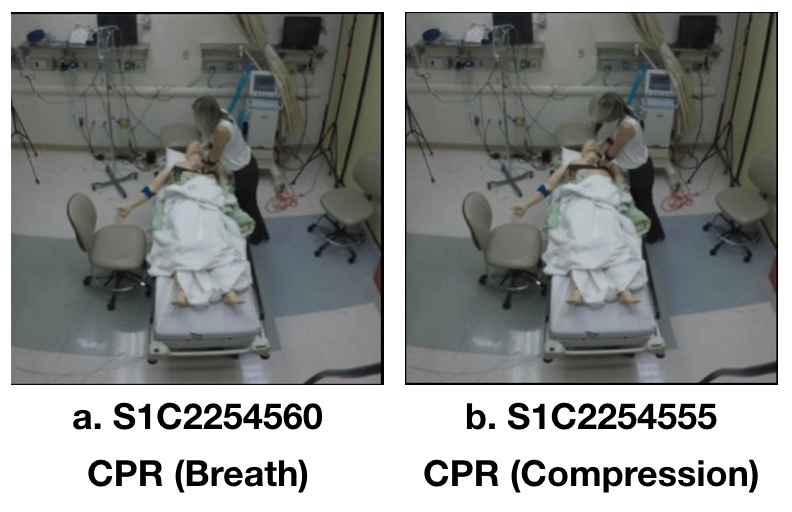
\includegraphics[width=25em]
        {./Fg5.png}}
        \caption{\label{fig: CPR Transition}  Similarity between CPR (Breath) (left) and CPR (Compression) (right). }
      \end{figure}

One cause of such inability is the close temporal proximity and the repetitiveness of the two categories. Compression and breath regularly happen one after another multiple times, and one major part of the CPR sequence is the transition time from one to the other. During data labeling, it is logical to randomly select a point in the transition and mark the division between two categories; however, during training, such an indistinct boundary between the two categories will cause confusion for the model. Figure~7 is an example of such problem. While both Figure~7a and Figure~7b come from the same transition period and they share significant similarity, Figure~7a is labeled as \textit{CPR (Breath)}, but Figure~7b is labeled as \textit{CPR (Compression)}. 

Such confusion is avoidable. The hospital may not benefit from knowing how many times compression is applied versus that of breath, so it makes sense to combine the two categories and report CPR as one category, and the similar logic also applies to \textit{Chest-tube} and \textit{Chest-tube Prep}, discussed next.

\begin{table}[!htb]
\begin{center}
 \begin{tabular}{||l c ||} 
 \hline
Category & Percentage \\ [0.5ex] 
 \hline\hline
Chest-tube & 59.678\%  \\ 
 \hline
IM Administration & 24.552\%  \\ 
  \hline
Suturing & 10.866\%  \\ 
 \hline
Others & 4.904\%  \\ 
 \hline
\end{tabular}
\caption{Table 5: Sorted misclassification categories for chest-tube prep.}
%5 fold , main model
\end{center}
\end{table}

Category \textit{Chest-tube Prep} stands out among other categories, because it consistently has accuracy near zero for all models. Table 5 shows the sorted categories to which models wrongly classify data of \textit{Chest-tube Prep}. The data suggests that for the majority of the time, models classify data from \textit{Chest-tube Prep} as \textit{Chest-tube} (59.678\%). It suggests that \textit{Chest-tube} and \textit{Chest-tube Prep} also suffer from the ambiguity problem during category transitions, as these two categories' occurrences are highly correlated. In addition, other factors such as the imbalance of data across subjects also potentially contribute to the low accuracy of \textit{Chest-tube Prep}. There are 10,262 frames of data available for \textit{Chest-tube Prep}; however,  two out of seven subjects do not contain any data, while  two subjects contains more than 6,000 frames of data. 


From the model size's stand point, due to the fact that variant 2 (the late fusion model) only uses a partial InceptionV3 model up to ``mixed6'' layer, and the parameters are shared across all branches, the number of the parameters used by the this model ($\approx$ 14M parameters) is significantly less than that used by the main model ($\approx$ 24M parameters). The reduced number of parameters, however, does not suggest that variant 2 requires less computation power than main model. 

Both variant 1 and variant 2 explore ideas to increase the performance of CNN based video classification methods for clinical procedures. The results and confusion matrices generated by main model, variant 1, and variant 2 give us suggestions for more practical ways of categorizing data and directions to create more powerful models. 

\section{Future Work}

In this work, we show that video classification methods from deep learning provide a tool for clinical procedure detection, potentially enhancing the communication between EMS and receiving hospitals. Future work includes training with improved data sets suggested by this work, incorporating data from multiple sensors into this framework as in Heard et al. [2], and trying improved deep learning models. The ultimate goal is to have models that work on video gathered in the field that can automatically detect clinical procedures to medically useful standards in real time.

New deep learning models for video classification are continually emerging. As part of this work, we tried a CNN-LSTM model, similar to work by Ng et al. [6], but were not able to get satisfactory results. Also of note, Feichtenhofer et al. [9] have just made available their SlowFast network, which recently had high performance on a video benchmark. As deep learning models improve, we expect our own identification results to improve.

%We have tried CNN-LSTM model to take advantage of temporal relations over a long period; however, probably due to the setting of LSTM model or the imperfection of CNN model weights, we are not able to get good results for it. Except a few occasions, We are not able to get the model to converge, training accuracies stay at low twenties until the end of the training sessions. It is interesting how we are not able to train CNN-LSTM model, and there may be some reasons we have not discovered yet. We will keep looking into LSTM for clinical procedure detection in the future.

%Last but not least, Feichtenhofer et al. [9] just open sourced their code for SlowFast network, which achieved state-of-the-art accuracy on major video recognition benchmark. We are interested to explore the capability of SlowFast network and observe how it performs on clinical procedure detection dataset.




%%%%%



%%%%%



%%%%%

\section*{ACKNOWLEDGMENTS}

The authors thank Kaiwen Xu for helpful suggestions. 


%%%%%



\begin{thebibliography}{99}

\bibitem{c1} M. K. James, L. A. Clarke, R. M. Simpson, A. J. Noto, J. R. Sclair, G. K. Doughlin, and S.-W. Lee, “Accuracy of pre-hospital trauma notification calls,” in \textit{The American Journal of Emergency Medicine}, 2018. 

\bibitem{c2} J. Heard, R. A. Paris, D. Scully, C. McNaughton, J. M. Ehrenfeld, J. Coco, D. Fabbri, B. Bodenheimer, "Automatic Clinical Procedure Detection for Emergency Services,"  in \textit{2019 41st Annual International Conference of the IEEE Engineering in Medicine and Biology Society (EMBC)}, Berlin, Germany, 2019, pp. 337-340. doi: 10.1109/EMBC.2019.8856281

\bibitem{c3} O. D. Lara and M. A. Labrador, “A survey on human activity recognition using wearable sensors,” in \textit{IEEE Communications on Surveys and Tutorials}, vol. 15, no. 3, pp. 1192–1209, 2013. 

\bibitem{c4} S. Ebrahimi Kahou, V. Michalski, K. Konda, R. Memisevic, and C. Pal. 2015. "Recurrent neural networks for emotion recognition in video," in \textit{Proceedings of the 2015 ACM on International Conference on Multimodal Interaction}. 467-474. ACM

\bibitem{c5} J. Donahue, L. Anne Hendricks, S. Guadarrama, M. Rohrbach, S. Venugopalan, K. Saenko, and T. Darrell. 2015. "Long-term recurrent convolutional networks for visual recognition and description," in \textit{Proceedings of the IEEE Conference on Computer Vision and Pattern Recognition.} 2625-2634

\bibitem{c6} Y.H. Ng, M. Hausknecht, S. Vijayanarasimhan, O. Vinyals, R. Monga, and G. Toderici. "Beyond Short Snippets: Deep Networks for Video Classification," in \textit{Proceedings of the Computer Vision \& Pattern Recognition, Boston}, MA, USA, 7–12 June 2015.

\bibitem{c7} R. A. Paris, P. Sullivan , J. Heard, D. Scully, C. McNaughton, J. M. Ehrenfeld, J. A. Adams, J. Coco, D. Fabbri, and B. Bodenheimer (2019, March). "Heatmap generation for emergency medical procedure identification" in \textit{Medical Imaging 2019: Image-Guided Procedures, Robotic Interventions, and Modeling} (Vol. 10951, p. 1095130). International Society for Optics and Photonics.

\bibitem{c8} A. Karpathy, G. Toderici, S. Shetty, T. Leung, R. Sukthankar, and F. Li. (2014). "Large-scale video classification with convolutional neural networks," in \textit{Proceedings of the IEEE conference on Computer Vision and Pattern Recognition} pp. 1725-1732.

\bibitem{c9} C. Feichtenhofer , H. Fan, J. Malik,  and K. He  (2019). "Slowfast networks for video recognition," in \textit{Proceedings of the IEEE International Conference on Computer Vision} pp. 6202-6211

\bibitem{c10} C. Szegedy, V. Vanhoucke, S. Ioffe, J. Shlens, and  Z. Wojna (2016). "Rethinking the inception architecture for computer vision" in \textit{Proceedings of the IEEE conference on computer vision and pattern recognition} pp. 2818-2826.



\end{thebibliography}




\end{document}
